% !TeX root = RJwrapper.tex
\title{A Review of R Neural Network Packages (with
\pkg{NNbenchmark})\(:\) Accuracy and Ease of Use}
\author{by Salsabila Mahdi, Akshaj Verma, Christophe Dutang, Patrice
Kiener, and John C. Nash}

\maketitle


\hypertarget{abstract}{%
\subsection{Abstract}\label{abstract}}

In the last three decades, neural-networks have evolved from an academic
topic to a common scientific computing tool. CRAN currently hosts around
80 packages (May 2020) that involve neural-network modeling; some
offering more than one algorithm. However, to our knowledge, there is no
comprehensive study which tests the accuracy, the reliability, and the
ease-of-use of those NN packages.

In this paper, we test a large number of packages against a common set
of datasets with varying levels of complexity to benchmark and rank them
with statistical metrics.

We restrict our evaluation to single hidden-layer perceptrons that
perform regression. We ignore packages for classification and other
specialized purposes. This leaves us with approximately 60
\code{package:algorithm} pairs to test. The criteria used in our
benchmark were: (i) accuracy, i.e.~the ability to find the global minima
on 13 datasets, measured by the Root Mean Square Error (RMSE) in a fixed
number of iterations; (ii) speed of the training algorithm; (iii)
availability of helpful utilities; (iv) quality of the documentation.

We have given a score for each evaluation criterion to compare all
\code{package:algorithm} pairs in a global table. Overall, 15 pairs are
considered accurate and reliable and are recommended for daily usage.
Other packages are either less accurate, slow, difficult to use, or have
poor or zero documentation.

To carry out this work, we developed multiple scripts along with the
\CRANpkg{NNbenchmark} package. We have open-sourced our code for
reproducibility on a github repository
\url{https://github.com/pkR-pkR/NNbenchmarkTemplates} as well as outputs
per package at \url{https://akshajverma.com/NNbenchmarkWeb/index.html}.

\hypertarget{introduction}{%
\subsection{Introduction}\label{introduction}}

The R Project for Statistical Computing, as any open-source platform,
relies on its contributors to keep it up to date. Neural Networks,
inspired by the brain itself, are a class of models in the growing field
of machine learning for which R has a number of tools. Previously,
neural networks were often considered theoretically instead of
pragmatically, partly because the algorithms used were computationally
expensive.

The term ``neural-network'' is colloquially used for different model
structures and applications. For regression and classification, the term
multilayer perceptron is used interchangeably. The term ``Recurrent
Neural Network'' is mainly used in the context of autoregressive
time-series while the term ``Convolutional Neural Networks'' for
dimension reduction and pattern recognition (images/audio/text). Most of
the above types of neural networks can be found in R packages hosted on
CRAN but without any study about the accuracy or the speed of
computation. This is an issue as many slow or poor algorithms are
available in the literature and hence poor packages are implemented on
CRAN.

A neural network algorithm requires complicated calculations to improve
the model control parameters. As with other optimization problems, the
gradient of the chosen cost function indicates the model's lack of
suitability. Optimization methods improve the current iterate by
changing the parameters in the opposite of the gradient direction
generally with an adaptive step. Parameters for the model are generally
obtained by using part of the available data (a training set) and tested
on the remaining data. Modern software allows much of this work,
including approximation of the gradient, to be carried out without a
large effort by the user.

The training process can generally be made more efficient if we can also
approximate second derivatives of the cost function, allowing us to use
its curvature via the Hessian matrix. There are a large number of
approaches, of which quasi-Newton algorithms are perhaps the most common
and useful. Within this group, methods based on the
Broyden-Fletcher-Goldfarb-Shanno (BFGS) algorithm for updating the
(inverse) Hessian approximation provide several well-known examples. In
conducting this study, we hypothesize that these second-order algorithms
would perform better than the first-order methods for datasets that fit
in memory.

To test our hypothesis, we conduct a thorough examination of these
training algorithms in R. There are many packages, but there's a dearth
of information that would allow the users to make an informed decision.
Our work aims to provide a framework for benchmarking neural-network
packages. We focus our examination to neural networks of the perceptron
type which consist of one input layer, one normalized layer, one hidden
layer with a non-linear activation function which is usually the
hyperbolic tangent \(\tanh()\), and one output layer.

Specifically, we focus only on regression based algorithms. The criteria
used in our benchmark were: (i) accuracy, i.e.~the ability to find the
global minima on 13 datasets, measured by the Root Mean Square Error
(RMSE) in a fixed number of iterations; (ii) speed of the training
algorithm; (iii) availability of helpful utilities; (iv) quality of the
documentation.

\hypertarget{neural-networks-the-perceptron}{%
\section{Neural Networks: The
Perceptron}\label{neural-networks-the-perceptron}}

In this section, we briefly describe the single hidden-layer perceptron.
As the ``layer'' term suggests - some terms come from graphs
representations while others come from the traditional literature on
non-linear models.

Using the graph description, a single-hidden layer neural network is
made up of 3 parts: (i) layer of the input(s), (ii) hidden layer which
consists of independent neurons, each of them performing two operations:
a linear combination of the inputs plus an offset followed by a
non-linear function, (iii) output layer which is a linear combination of
the output of the previous layer.

The non-linear function used in the hidden layer must have the following
four properties: continuous, differentiable, monotonic, and bounded. The
logistic (\(\text{invlogit}\)), hyperbolic tangent (\(\tanh\)) and
arctangent (\(\text{atan}\)) functions are the usual candidates. The
above description has a simple mathematical equivalence. Let us take two
examples.

The model
\(y = a_1 + a_2\times \tanh(a_3 + a_4\times x) + a_5\times \tanh(a_6 + a_7\times x) + a_8\times \tanh(a_9 + a_{10}\times x)\)
describes a neural network (Fig. 1a) with one input, three hidden
neurons, one output model where \(x\) is the input, \(\tanh()\) is the
activation function, \(y\) is the output and \(a_1,\dots,a_{10}\) are
the parameters.

The model
\(y = a_1 + a_2\times \text{atan}(a_3 + a_4\times x_1 + a_5\times x_2 + a_6\times x_3 + a_7\times x_4 + a_8\times x_5) + a_9\times \text{atan}(a_{10} + a_{11}\times x_1 + a_{12}\times x_2 + a_{13}\times x_3 + a_{14}\times x_4 + a_{15}\times x_5) + a_{16}\text{atan}(a_{17} + a_{18}\times x_1 + a_{19}\times x_2 + a_{20}\times x_3 + a_{21}\times x_4 + a_{22}\times x_5)\)
describes a neural network (Fig. 1b) with five inputs, three hidden
neurons, one output model where \(x\) is the input, \(\text{atan}()\) is
the activation function, \(y\) is the output and \(a_1,\dots,a_{22}\)
are the parameters.

While the final gradient should be small, we believe it is helpful to
have relatively large gradients at the first steps of the training
algorithm, so the following is recommended: (i) normalized inputs and
outputs (Fig. 1c), (ii) odd functions like the hyperbolic tangent
function or the arctangent function, (iii) small random values to
initialize the parameters. A common example of this is to use values
extracted from a centred Gaussian \(\mathcal N(0, 0.1)\) distribution.

These practices help us find good local-minima and possibly the
global-minima.

\begin{figure}
    \centering
    \begin{subfigure}[b]{0.242\textwidth}
        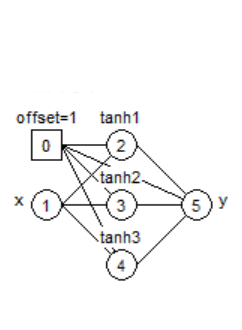
\includegraphics[width=\textwidth]{RN3a2.png}
        \caption{NN 1-3-1}
        \label{fig:N131}
    \end{subfigure}
    ~ 
    \begin{subfigure}[b]{0.250\textwidth}
        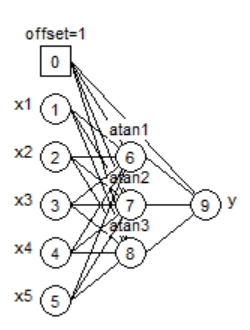
\includegraphics[width=\textwidth]{RN3b2.png}
        \caption{NN 5-3-1}
        \label{fig:N531}
    \end{subfigure}
    ~ 
    \begin{subfigure}[b]{0.396\textwidth}
        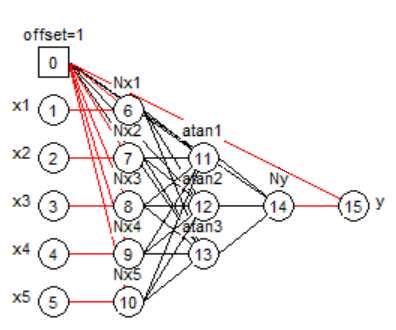
\includegraphics[width=\textwidth]{RN3c2.png}
        \caption{NN 5-5N-3-1N-1}
        \label{fig:N55311}
    \end{subfigure}
    \caption{Three neural networks}
\end{figure}

The dataset used for the training is assumed to have the number of rows
much larger than the number of parameters. While ``much larger'' is
subjective, values of 3 to 5 are generally accepted (in experimental
design, some iterative strategies start with a dataset having a number
of distinct experiments equal to 1.8 times the number of parameters and
then increase the number of experiments to fine tune the model).

It is rather clear from the mathematical formula above that neural
networks of perceptron type are non-linear models which require training
algorithms that can handle (highly) non-linear models for their
parameter estimation. Indeed, the intrinsic and parametric curvatures of
such models are usually very high and with so many parameters, the
Jacobian matrix might exhibit some co-linearities between its columns
and become nearly singular. As a result, appropriate algorithms for such
\code{dataset::model} pairs are rather limited and well-known. They
pertain to the class of second-order algorithms such as the BFGS
algorithm which is Quasi-Newton in how it updates the approximate
inverse Hessian or the Levenberg-Marquardt algorithm which stabilizes
the Gauss-Newton search direction at every iteration.

Unfortunately, due to certain educative tools on the backpropagation and
recent popularity of ``deep neural networks'' that manipulate
ultra-large models (sometimes more parameters than examples in the
datasets), many papers emphasize the use of first-order gradient
algorithms.

Therefore, many R packages have implemented such algorithms. In the case
of the perceptron, we contend this is an oversight, and provide evidence
to that effect in this paper. We refer interested readers to
\citep{tan2019review} for a review of second-order algorithms for neural
networks.

\hypertarget{methodology}{%
\section{Methodology}\label{methodology}}

\hypertarget{convergence-and-termination}{%
\subsection{Convergence and
termination}\label{convergence-and-termination}}

Most of the \code{package:algorithm} pairs try to minimize the Root Mean
Squared Error (RMSE) during the training step. Two exceptions are the
\CRANpkg{brnn} package which minimizes the RMSE plus the sum of the
parameters (hence the name Bayesian Regularized Neural Network), and the
\CRANpkg{qrnn} package which performs quantile regression. For all
packages, the datasets were learnt as a whole and without any weighting
scheme to favor a single part of a dataset. We don't use a
validation/test set because the purpose of our study is to verify the
ability to reach good minima. This requirement is satisfied by using
only a train set.

When training neural networks, we attempt to tune a set of
hyperparameters so that the root to minimize the RMSE. When our method
for such adjustment can no longer reduce the RMSE, we say that the given
algorithm \textbf{terminated}. We consider the method to have
\textbf{converged} when termination is not due to some exceptional
situation and the final RMSE value is relatively small\footnote{We do
  not choose the mean absolute error (MAE) for overall ranking nor for
  convergence testing as there is a lack of consensus in the literature,
  see e.g.~\citep{willmott2005advantages,chai2014root}.}. In practice,
some algorithms require that we stop the optimization process in
exceptional situations (e.g., a divide by zero), or a pre-set limit on
the number of steps or a maximum elapsed time is reached.

Specifically, second-order algorithms are all set to a maximum of 200
iterations. On the other hand, first-order algorithms were set to
several values, depending on how well and how fast they converged:
\texttt{maxit1storderA=1000} iterations, \texttt{maxit1storderB=10000}
iterations, and \texttt{maxit1storderC=100000} iterations. The full list
of the maximum iteration number per \code{package:algorithm} is given in
Table 4 in Appendix D. It can be seen that we were unable to completely
harmonize the hyperparameters as an appropriate learning rate differed
between packages, despite the algorithm being similarly named.

\hypertarget{performance}{%
\subsection{Performance}\label{performance}}

We measure \textbf{performance} primarily by relative computing time
between methods on a particular computing platform. We could count the
precise number of iterations, function evaluations or similar quantities
that indicate the computing effort, but this would have required a large
effort in R coding in order to get values that are comparable between NN
packages. We note that differences in machine architecture and in the
attached libraries (e.g., BLAS choices for R) will modify our
performance measure. We are putting our tools on a Github repository so
that further evaluation can be made by ourselves and others as hardware
and software evolves.

The majority of the resulting files in our repository were generated on
a Windows system build 10.0.18362.752. The machine specifications are -
(i) i7-8750H CPU, (ii) Intel(R) UHD Graphics 630, (iii) NVIDIA GeForce
GTX 1060 chip, (iv) 16 GB of RAM.

Tests were also performed on other platforms and the computation times
were found to be reasonably similar.

\hypertarget{phase-1---preparation-of-benchmark-datasets-and-selection-of-packages}{%
\subsection{Phase 1 - Preparation of benchmark datasets and selection of
packages}\label{phase-1---preparation-of-benchmark-datasets-and-selection-of-packages}}

\textbf{Datasets}

A non-iterative calculation such as Ordinary Least Squares cannot
generally be used to model all the datasets in our evaluation set.
Varying levels of difficulty in modeling the different data sets are
intended to allow us to further classify different algorithms and the
packages that implement them. As we focus on regression analysis, we
select only datasets where the response variable is real-valued.

Sonja Surjanovic and Derek Bingham of Simon Fraser University created a
useful website from which three of the multivariate datasets were drawn.
We note the link, name and difficulty level of the three datasets:

\begin{itemize}
\tightlist
\item
  \url{http://www.sfu.ca/~ssurjano/fried.html}: \code{mFriedman},
  Friedman's dataset, published in \citep{friedman91} (average
  difficulty),\\
\item
  \url{http://www.sfu.ca/~ssurjano/detpep10curv.html}: \code{mDette},
  Dette's dataset, published in \citep{dettePepelyshev10} (medium
  difficulty),\\
\item
  \url{http://www.sfu.ca/~ssurjano/ishigami.html}: \code{mIshigami},
  Ishigami's dataset, published in \citep{ishigamietal90} (high
  difficulty).
\end{itemize}

The last multivariate dataset, \code{mRef153}, was used to teach neural
networks at ESPCI (The City of Paris Industrial Physics and Chemistry
Higher Educational Institution, \url{https://www.neurones.espci.fr/})
from 2003 to 2013 and is available in the proprietary software Neuro One
at \url{http://www.inmodelia.com/software.html}. This dataset presents
some interesting non-linear features.

\code{uDreyfus1} is a pure neural network which has no error. This can
make it difficult for algorithms that assume an error exists.
\code{uDreyfus2} is \code{uDreyfus1} with errors. Both are considered to
be of low difficulty and used to teach neural networks at ESPCI from
1991 to 2013. \code{uDmod1} and \code{uDmod2} are univariate datasets
with few observations but exhibit high non-linear patterns and prove to
be very challenging datasets. The parameters are highly correlated and
singular Jacobian matrices often appear.

Three of the univariate datasets were taken from the US National
Institute for Standards and Technology (NIST) website:
\url{https://www.itl.nist.gov/div898/strd/nls/nls_main.shtml}. Namely
\code{uGauss1}, \code{uGauss2} and \code{uGauss3} published in
\citep[resp.]{rustnist96:Gauss1,rustnist96:Gauss2,rustnist96:Gauss3}
created by NIST to assess non-linear least squares regressions are of
low, low and medium difficulty respectively.

The last univariate dataset, \code{uNeuroOne}, was also used to teach
the same course and is now available in the proprietary software
NeuroOne at \url{http://www.inmodelia.com/software.html}. In Table 1, we
list some information on each dataset used in the first round of our
analysis: the number of neurons and the induced parameter number are
available in the last two columns.

\begin{Schunk}
\begin{table}

\caption{\label{tab:unnamed-chunk-2}Datasets' summary}
\centering
\fontsize{7}{9}\selectfont
\begin{tabular}[t]{lcccc}
\toprule
Dataset & Row nb. & Input nb. & Neuron nb. & Param. nb.\\
\midrule
\addlinespace[0.3em]
\multicolumn{5}{l}{\textbf{Multivariate}}\\
\hspace{1em}mDette & 500 & 3 & 5 & 26\\
\hspace{1em}mFriedman & 500 & 5 & 5 & 36\\
\hspace{1em}mIshigami & 500 & 3 & 10 & 51\\
\hspace{1em}mRef153 & 153 & 5 & 3 & 22\\
\addlinespace[0.3em]
\multicolumn{5}{l}{\textbf{Univariate}}\\
\hspace{1em}uDmod1 & 51 & 1 & 6 & 19\\
\hspace{1em}uDmod2 & 51 & 1 & 5 & 16\\
\hspace{1em}uDreyfus1 & 51 & 1 & 3 & 10\\
\hspace{1em}uDreyfus2 & 51 & 1 & 3 & 10\\
\hspace{1em}uGauss1 & 250 & 1 & 5 & 16\\
\hspace{1em}uGauss2 & 250 & 1 & 4 & 13\\
\hspace{1em}uGauss3 & 250 & 1 & 4 & 13\\
\hspace{1em}uNeuroOne & 51 & 1 & 2 & 7\\
\bottomrule
\end{tabular}
\end{table}

\end{Schunk}

Finally, we consider a Simon Wood test dataset, named \code{bWoodN1},
used in \citep{wood2011fast} for benchmarking generalized additive
models. Precisely, we consider a generation of Gaussian random variates
\(Y_i\), \(i=1,\dots,n\) with the mean \(\mu_i\) defined as \[
\mu_i = 1+ f_0(x_{i,0})+f_1(x_{i,1})+f_2(x_{i,2})+f_3(x_{i,3})
+f_4(x_{i,4})+f_0(x_{i,5})
\] and standard deviation \(\sigma=1/4\) where \(f_j\) are Simon Wood's
smooth functions defined in Appendix B, \(x_{i,j}\) are uniform variates
and \(n=20,000\). \code{bWoodN1} will only be used in the second round
of our analysis when the TOP-5 packages will be further analyzed with 5
neurons resulting in 41 parameters.

To build the final result table, we selected all four multivariate
datasets and 4 out of the 8 univariate datasets so that the overall
score does not overly weight the univariate datasets. Note that the 2020
GSoC results are available in Section 1 of the supplementary materials,
\citep{suppl:material:paper}. Furthermore the 2019 GSoC code uses all 12
datasets. For convenience, all datasets are made available in
\CRANpkg{NNbenchmark}, so that anyone can replicate our analysis.

\textbf{Packages}

Using \CRANpkg{RWsearch} \citep{R-RWsearch}, we sought to automate the
process of searching for neural network packages. All packages that have
``neural network'' as a keyword in the package title or in the package
description were included.

As of May 2020, around 80 packages fall into this category. Packages
\CRANpkg{nlsr}, \CRANpkg{minpack.lm}, \CRANpkg{caret} were added because
the former two are important implementations of second-order algorithms
while the latter is the first cited meta package in the CRAN task view
for machine learning, \ctv{MachineLearning}. It is also a dependency for
some of the other packages tested. Restricting to regression analysis
left us with 49 \code{package:algorithm} pairs in 2019 and 60
\code{package:algorithm} pairs in 2020.

\hypertarget{phase-2---review-of-packages-and-development-of-a-benchmarking-template}{%
\subsection{Phase 2 - Review of packages and development of a
benchmarking
template}\label{phase-2---review-of-packages-and-development-of-a-benchmarking-template}}

All packages were tested 3 times. Each assessment is described in detail
below.

\textbf{1. The decision to exclude or include}

From documentation and example code, we learned that not all packages
selected by the automated search fit the scope of our research. Some
have no function to generate neural networks while others were not
regression neural networks of the perceptron type or were only intended
for very specific purposes: for instance to predict the amyloidogenicity
propensity of polypeptide sequences. Depending on the package, this
could be decided by looking at the \code{DESCRIPTION} file or by trial
and error.

\textbf{2. Templates for testing accuracy and speed}

While inspecting the packages, we slowly developed a template for
benchmarking that evolved over time. The final structure of this
template (for each package) is as follows:

\begin{enumerate}
\def\labelenumi{\arabic{enumi}.}
\tightlist
\item
  Set up the test environment - loading of packages, setting working
  directory and options;
\item
  Summary of tested datasets;
\item
  Loop over datasets:

  \begin{enumerate}
  \def\labelenumii{\alph{enumii}.}
  \tightlist
  \item
    setting parameters for a specific dataset,
  \item
    selecting benchmark options,
  \item
    training a neural network with a tuned function for each package,
  \item
    calculation of convergence metrics (RMSE, MAE, WAE)\footnote{We
      measure the quality of our model by RMSE, but the mean absolute
      error (MAE) and the worst absolute error (WAE) may help
      distinguish packages with close RMSE values. See Appendix A for
      definition of convergence metrics.},
  \item
    plot each training over one initial graph, then plot the best
    result,
  \item
    add results to the appropriate existing record (*.csv file) and
  \item
    clear the environment for next loop.
  \end{enumerate}
\item
  Clearing up the environment for the next package. It is optional to
  print warnings.
\end{enumerate}

To simplify this process, we developed tools in the \pkg{NNbenchmark}
package, of which the first version was created as part of GSoC'19. In
GSoC'20, 3 functions encapsulating the template were added that have
been made generic with the extensive use of the \code{do.call} function
from the \pkg{base} package:

\begin{enumerate}
\def\labelenumi{\arabic{enumi}.}
\tightlist
\item
  In \code{trainPredict\_1mth1data} a neural network is trained on one
  dataset and then used for predictions, with several utilities. Then
  the performance of the neural network is exported, plotted and/or
  summarized.
\item
  \code{trainPredict\_1data} serves as a wrapper function for
  \code{trainPredict\_1mth1data} for multiple methods.
\item
  \code{trainPredict\_1pkg} serves as a wrapper function for
  \code{trainPredict\_1mth1data} for multiple datasets.
\end{enumerate}

A function for the summary of accuracy and speed, \code{NNsummary}, was
also added. The package repository is at
\url{https://github.com/pkR-pkR/NNbenchmark}, with template repository
at \url{https://github.com/pkR-pkR/NNbenchmarkTemplates}, and outputs
per package at \url{https://akshajverma.com/NNbenchmarkWeb/index.html}.
An example of a call to \code{trainPredict\_1pkg} is given in Appendix
C.

\textbf{3. Ease of use scoring}

We define ease-of-use measures to rate NN packages on their
user-friendliness. Based on our understanding of what a user may be
required to know or do when using a neural network package, we consider:
(i) a measure for the availability of appropriate utility functions (ii)
a measure for (non-trivial) examples (iii) a sufficient documentation
(well-written manual, vignette(s)) (iv) a measure to rate the clarity of
the R call to fit a given neural network.

Our ratings are as follows.

\begin{enumerate}
\def\labelenumi{\arabic{enumi}.}
\tightlist
\item
  Utilities in R to deal with NN

  \begin{enumerate}
  \def\labelenumii{\alph{enumii}.}
  \tightlist
  \item
    a predict function exists = 1 star
  \item
    scaling capabilities exist = 1 star
  \end{enumerate}
\item
  Sufficient and reliable documentation

  \begin{enumerate}
  \def\labelenumii{\alph{enumii}.}
  \tightlist
  \item
    the existence of useful and relevant example(s)/vignette(s)

    \begin{itemize}
    \tightlist
    \item
      clear, with regression = 2 stars
    \item
      unclear, examples use iris or are for classification only = 1 star
    \item
      no examples = 0 stars
    \end{itemize}
  \item
    input/output is clearly documented, e.g., what values are expected
    and returned by a function

    \begin{itemize}
    \tightlist
    \item
      clear input and output = 2 stars
    \item
      only one is clear = 1 star
    \item
      both are not documented = 0 stars
    \end{itemize}
  \end{enumerate}
\item
  User-friendly call to fit a NN

  \begin{enumerate}
  \def\labelenumii{\alph{enumii}.}
  \tightlist
  \item
    simple one-line call or a single function = 2 stars
  \item
    multiple-lines call to a single function = 1 star
  \item
    multiple-lines call to many functions = 0 stars
  \end{enumerate}
\end{enumerate}

Hence, to inform users about the usability of packages, the
documentation measure ranges from 0 to 4 stars, while the utility and
the R call range from 0 to 2 stars.

\hypertarget{phase-3---collection-of-and-analysis-of-results}{%
\subsection{Phase 3 - Collection of and analysis of
results}\label{phase-3---collection-of-and-analysis-of-results}}

\hypertarget{results-collection}{%
\subsubsection{Results collection}\label{results-collection}}

Looping over the datasets using each package template, we collected
results in the relevant package directories that rests in the templates
repository. A large number of runs were carried out in order to obtain
the best result for every package.

\hypertarget{analysis}{%
\subsubsection{Analysis}\label{analysis}}

To rank the speed and quality of convergence, we have devised the
following method:

\begin{enumerate}
\def\labelenumi{\arabic{enumi}.}
\tightlist
\item
  The results datasets are loaded into the R environment as one large
  list. The dataset names, \code{package:algorithm} names and all 10 run
  numbers, durations, and RMSE are extracted from that list.
\item
  For the duration score (DUR), the duration is averaged by dataset. 3
  criteria for the RMSE score by dataset are calculated:

  \begin{enumerate}
  \def\labelenumii{\alph{enumii}.}
  \tightlist
  \item
    The minimum value of RMSE for each \code{package:algorithm} as a
    measure of their best performance;
  \item
    The median value of RMSE for each \code{package:algorithm} as a
    measure of their average performance, without the influence of
    outliers;
  \item
    The spread of the RMSE values for each package which is measured by
    the difference between the median and the minimum RMSE (subsequently
    referred to as RMSE D51).
  \end{enumerate}
\item
  Then, the ranks are calculated for every dataset and the results are
  merged into one wide dataframe.

  \begin{enumerate}
  \def\labelenumii{\alph{enumii}.}
  \tightlist
  \item
    The duration rank only depends on the duration;
  \item
    For minimum RMSE values, ties are decided by duration mean, then the
    RMSE median;
  \item
    For median RMSE values, ties are decided by the RMSE minimum, then
    the duration mean;
  \item
    The RMSE D51 rank only depends on itself.
  \end{enumerate}
\item
  A global score for all datasets is found by a sum of the ranks (of
  duration, minimum RMSE, median RMSE, RMSE D51) of each
  \code{package:algorithm} for each dataset.
\item
  The final table is the result of ranking by the global minimum RMSE
  scores for each \code{package:algorithm}.
\end{enumerate}

\hypertarget{results-discussion-and-recommendations}{%
\section{Results, discussion and
recommendations}\label{results-discussion-and-recommendations}}

Table 2 gives the RMSE and time score per package and per algorithm. The
full list of scores is given in Table 4 in Appendix D. We divide our
analysis in two groups: packages implementing second-order algorithms
and packages implementing first-order algorithms. Figure 2 shows the
minimum RMSE value per \code{package:algorithm} for two particular
datasets \code{mIshigami} and \code{uDreyfus1}, whereas Figure 3
displays the average computation time. The number on the x-level refers
to the RMSE overall score of the \code{package:algorithm} given in Table
2 (last column), e.g., 8 refers to \code{validann:optim(CG)} which is a
very slow algorithm.

Both figures show that a good overall score does not necessarily imply a
good performance on the two datasets under consideration. Furthermore,
there is a break between the TOP-10 \code{package:algorithm} and others
in terms of RMSE value. In Section 1.13 of the supplementary materials,
\citep{suppl:material:paper}, the score probabilities per
\code{package:algorithm} also gives some insights how robust is the
overall score.

Regarding computation time, we observe that some
\code{package:algorithm} are very slow and have poor RMSE, e.g.~41
corresponding to \code{AMORE:BATCHgd}. In the following, we first
present the results for second-order algorithms, then low-order
algorithms. Finally, we list the reasons for discarded packages.

\begin{Schunk}
\begin{table}

\caption{\label{tab:unnamed-chunk-3}Result from Tested Packages}
\centering
\fontsize{7}{9}\selectfont
\begin{tabular}[t]{>{}lccclc>{}c}
\toprule
\multicolumn{1}{c}{ } & \multicolumn{3}{c}{Individual rating} & \multicolumn{1}{c}{ } & \multicolumn{2}{c}{Global score} \\
\cmidrule(l{3pt}r{3pt}){2-4} \cmidrule(l{3pt}r{3pt}){6-7}
Package & Util & Doc & Call & Algorithm & Time & RMSE\\
\midrule
\textbf{nlsr} & * & **** & ** & 41. NashLM & 18 & \textbf{1}\\
\cmidrule{1-7}
\textbf{rminer} & ** & *** & ** & 45. nnet\_optim(BFGS) & 12 & \textbf{2}\\
\cmidrule{1-7}
\textbf{nnet} & * & *** & ** & 42. optim (BFGS) & 3 & \textbf{3}\\
\cmidrule{1-7}
 & * & **** & ** & 56. optim(BFGS) & 35 & \textbf{4}\\

 & * & **** & ** & 57. optim(CG) & 60 & \textbf{8}\\

 & * & **** & ** & 58. optim(L-BFGS-B) & 36 & \textbf{15}\\

 & * & **** & ** & 59. optim(Nelder-Mead) & 55 & \textbf{45}\\

\multirow{-5}{*}{\raggedright\arraybackslash \textbf{validann}} & * & **** & ** & 60. optim(SANN) & 20 & \textbf{55}\\
\cmidrule{1-7}
\textbf{MachineShop} & * & *** & * & 32. nnet\_optim(BFGS) & 6 & \textbf{5}\\
\cmidrule{1-7}
\textbf{traineR} & * & ** & ** & 55. nnet\_optim(BFGS) & 4 & \textbf{6}\\
\cmidrule{1-7}
\textbf{radiant.model} & ** & ** & ** & 44. nnet\_optim(BFGS) & 10 & \textbf{7}\\
\cmidrule{1-7}
 & ** & *** & ** & 34. optimx(BFGS) & 26 & \textbf{9}\\

\multirow{-2}{*}{\raggedright\arraybackslash \textbf{monmlp}} & ** & *** & ** & 35. optimx(Nelder-Mead) & 32 & \textbf{47}\\
\cmidrule{1-7}
 & ** & *** & ** & 12. optim(BFGS) & 46 & \textbf{10}\\

 & ** & *** & ** & 14. Rprop & 56 & \textbf{51}\\

\multirow{-3}{*}{\raggedright\arraybackslash \textbf{CaDENCE}} & ** & *** & ** & 13. pso\_psoptim & 54 & \textbf{54}\\
\cmidrule{1-7}
\textbf{h2o} & ** & ** &  & 24. first-order & 51 & \textbf{11}\\
\cmidrule{1-7}
\textbf{EnsembleBase} & * & * & ** & 23. nnet\_optim(BFGS) & 5 & \textbf{12}\\
\cmidrule{1-7}
\textbf{caret} & ** & *** & ** & 15. avNNet\_nnet\_optim(BFGS) & 17 & \textbf{13}\\
\cmidrule{1-7}
\textbf{brnn} & ** & **** & ** & 11. Gauss-Newton & 8 & \textbf{14}\\
\cmidrule{1-7}
\textbf{qrnn} & ** & *** & ** & 43. nlm() & 28 & \textbf{16}\\
\cmidrule{1-7}
 & ** & *** & ** & 51. Rprop & 24 & \textbf{17}\\

 & ** & *** & ** & 52. SCG & 30 & \textbf{18}\\

 & ** & *** & ** & 53. Std\_Backpropagation & 22 & \textbf{27}\\

 & ** & *** & ** & 47. BackpropChunk & 26 & \textbf{29}\\

 & ** & *** & ** & 48. BackpropMomentum & 25 & \textbf{30}\\

 & ** & *** & ** & 49. BackpropWeightDecay & 29 & \textbf{31}\\

 & ** & *** & ** & 46. BackpropBatch & 43 & \textbf{49}\\

\multirow{-8}{*}{\raggedright\arraybackslash \textbf{RSNNS}} & ** & *** & ** & 50. Quickprop & 45 & \textbf{57}\\
\cmidrule{1-7}
 & * & *** & ** & 8. trainwgrad\_adam & 50 & \textbf{18}\\

 & * & *** & ** & 9. trainwgrad\_RMSprop & 47 & \textbf{26}\\

\multirow{-3}{*}{\raggedright\arraybackslash \textbf{automl}} & * & *** & ** & 10. trainwpso & 57 & \textbf{43}\\
\cmidrule{1-7}
\textbf{deepnet} & * & *** & ** & 20. BP & 23 & \textbf{18}\\
\cmidrule{1-7}
 & * & *** & ** & 38. rprop+ & 19 & \textbf{21}\\

 & * & *** & ** & 37. rprop- & 21 & \textbf{22}\\

 & * & *** & ** & 40. slr & 31 & \textbf{31}\\

 & * & *** & ** & 39. sag & 41 & \textbf{38}\\

\multirow{-5}{*}{\raggedright\arraybackslash \textbf{neuralnet}} & * & *** & ** & 36. backprop & 37 & \textbf{50}\\
\cmidrule{1-7}
 & ** & * &  & 28. adamax & 48 & \textbf{23}\\

 & ** & * &  & 27. adam & 42 & \textbf{34}\\

 & ** & * &  & 29. nadam & 44 & \textbf{36}\\

 & ** & * &  & 26. adagrad & 58 & \textbf{37}\\

 & ** & * &  & 25. adadelta & 59 & \textbf{40}\\

 & ** & * &  & 31. sgd & 48 & \textbf{44}\\

\multirow{-7}{*}{\raggedright\arraybackslash \textbf{keras}} & ** & * &  & 30. rmsprop & 37 & \textbf{52}\\
\cmidrule{1-7}
 & * & *** & * & 2. ADAPTgdwm & 16 & \textbf{24}\\

 & * & *** & * & 1. ADAPTgd & 9 & \textbf{35}\\

 & * & *** & * & 4. BATCHgdwm & 40 & \textbf{39}\\

\multirow{-4}{*}{\raggedright\arraybackslash \textbf{AMORE}} & * & *** & * & 3. BATCHgd & 39 & \textbf{41}\\
\cmidrule{1-7}
\textbf{minpack.lm} & * & *** & ** & 33. Levenberg-Marquardt & 15 & \textbf{24}\\
\cmidrule{1-7}
 & ** & *** & * & 6. rmsprop & 14 & \textbf{28}\\

 & ** & *** & * & 5. adam & 13 & \textbf{33}\\

\multirow{-3}{*}{\raggedright\arraybackslash \textbf{ANN2}} & ** & *** & * & 7. sgd & 11 & \textbf{42}\\
\cmidrule{1-7}
 & ** & *** & ** & 16. adam & 32 & \textbf{46}\\

 & ** & *** & ** & 19. rmsProp & 34 & \textbf{53}\\

 & ** & *** & ** & 18. momentum & 53 & \textbf{56}\\

\multirow{-4}{*}{\raggedright\arraybackslash \textbf{deepdive}} & ** & *** & ** & 17. gradientDescent & 52 & \textbf{58}\\
\cmidrule{1-7}
\textbf{snnR} & ** & ** & ** & 54. SemiSmoothNewton & 7 & \textbf{48}\\
\cmidrule{1-7}
\textbf{elmNNRcpp} & ** & *** & ** & 21. ELM & 1 & \textbf{59}\\
\cmidrule{1-7}
\textbf{ELMR} & ** & *** & ** & 22. ELM & 2 & \textbf{60}\\
\bottomrule
\multicolumn{7}{l}{\rule{0pt}{1em}\textit{Note: } Statistics over 10 runs.}\\
\end{tabular}
\end{table}

\end{Schunk}

\begin{figure}
  \centering
  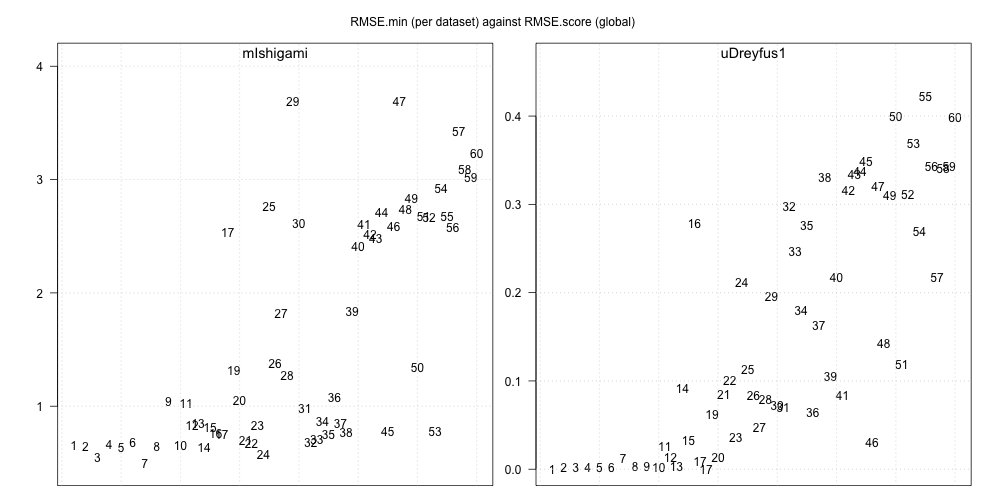
\includegraphics[width=\textwidth]{mIshigami-uDreyfus1-RMSEmin.png}
        \label{fig:Allpkg:RMSEmin}
        \caption{RMSE minimum value per package for \code{mIshigami}
        and \code{uDreyfus1} datasets}
\end{figure}

\begin{figure}
  \centering
  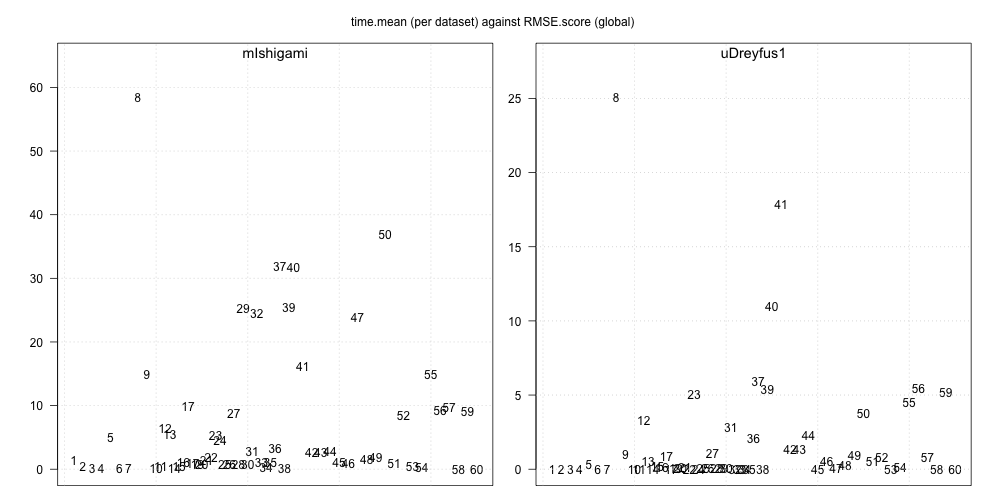
\includegraphics[width=\textwidth]{mIshigami-uDreyfus1-timmean.png}
        \label{fig:Allpkg:timemean}
        \caption{Average time value per package for \code{mIshigami}
        and \code{uDreyfus1} datasets}
\end{figure}

\hypertarget{second-order-algorithms}{%
\subsection{Second-order algorithms}\label{second-order-algorithms}}

Of all approaches, the following second-order algorithms generally
performed better in terms of convergence despite being limited to
\(1/5^{th}\) or fewer iterations than the first-order algorithms.

We note that 11 out of 15 of these \code{package:algorithms} use
\code{optim} from \pkg{stats}. 2 of them, \CRANpkg{CaDENCE}`s BFGS
\citep{R-CaDENCE} and \CRANpkg{validann}'s BFGS and L-BFGS-B
\citep{R-validann}, make the call directly. However, it is not clearly
stated in \pkg{CaDENCE}'s documentation that \code{optim}'s BFGS method
has been chosen rather than one of the other four methods. Furthermore,
the mention of Nelder-Mead in the documentation suggests that
\code{optim}'s Nelder-Mead method is used. Speed and variation between
results for \pkg{CaDENCE} are also not as good as other packages that
use \code{optim}. This could be because \pkg{CaDENCE} is intended for
probabilistic non-linear models with a full title of ``Conditional
Density Estimation Network Construction and Evaluation''.

By contrast, \pkg{validann} is clearly a package that allows a user to
use all \code{optim}'s algorithms. \pkg{validann}\code{:L-BFGS-B} ranks
mostly lower than \pkg{validann}\code{:BFGS}, despite the former method
being more sophisticated. We believe this is due to our efforts to
harmonize parameters, thereby under-utilizing the possibilities of the
L-BFGS-B algorithm. Both \pkg{CaDENCE} and \pkg{validann}'s BFGS are
outperformed by \CRANpkg{nnet}, especially in terms of speed.

\pkg{nnet} \citep{R-nnet} differs from the two packages above because it
uses the C code for BFGS (\code{vmmin.c}) from \code{optim} (converted
earlier from Pascal) directly instead of calling \code{optim} from R.
This may be what allows it to be faster, but limits the optimization to
the single method. \pkg{nnet} is only beaten by the Extreme Learning
Machine (ELM) algorithms in terms of speed. However, there is a larger
variation between results (see the \texttt{RMSE\ D51} in Appendix D) in
comparison to \pkg{validann}:BFGS. We believe the different default
starting values are the cause of this. For instance, \pkg{nnet} uses a
range of initial random weights of 0.7 while \pkg{validann} uses a value
of 0.5. In spite of these results, the real reason most authors or users
are likely to choose \pkg{nnet} is because it is included in the
distributed base R and is even mentioned as the very first package in
CRAN's task view for machine learning (\ctv{MachineLearning}).

Our analysis found that 6 out of 11 packages tested that use
\code{optim} do so through \pkg{nnet}. Moreover, approximately 8
packages for neural networks, though not tested, use \pkg{nnet}.

The total number of \pkg{nnet} dependencies found through a search
through the offline database of CRAN with \pkg{RWsearch} is 136
packages, although some might be using \pkg{nnet} for the multinomial
log-linear models, not neural networks.

The packages that use \pkg{nnet} for neural networks are often meta
packages with a host of other machine learning algorithms. \pkg{caret}
\citep{R-caret}, also mentioned in the task-view, boasts 238 methods
with 13 different neural network packages, under a deceivingly simple
name of ``Classification and Regression Training''. It has many
pre-processing utilities available, as well as other tools.

\CRANpkg{EnsembleBase} \citep{R-EnsembleBase} may be useful for those
who wish to make model ensembles and test a grid of parameters, although
the documentation is rather confusing. \CRANpkg{MachineShop}
\citep{R-MachineShop} has 51 algorithms, with some additional
information about the response variable types in the second vignette,
functions for preprocessing and tuning, performance assessment, and
presentation of results. \CRANpkg{radiant.model} \citep{R-radiant.model}
has an unalterable \code{maxit} of 10000 in the original package. We
changed this to harmonize the \code{maxit} parameter. \CRANpkg{rminer}
\citep{R-rminer} is the only package dependent on \pkg{nnet} that ranks
above \pkg{nnet} at number 2 for minimum RMSE, and even number 1 in some
runs. It also ranks number 1 on the other accuracy measures (median
RMSE, minimum MAE, minimum WAE) and is only behind \CRANpkg{deepdive}
and \pkg{minpack.lm} in terms of results that are consistent and do not
vary (RMSE D51).

The difference is probably from the change of maximum allowable weights
in \pkg{rminer} to 10000 from 1000 in \pkg{nnet}, which is also probably
the reason its fits are slower. \CRANpkg{traineR} \citep{R-traineR}
claims to unify the different methods of creating models between several
learning algorithms.

It is worth noting is that \pkg{nnet} and \pkg{validann} do not have
external normalization, which is especially recommended for
\pkg{validann}. However, some of the packages dependent on \pkg{nnet} do
have this capability and it is included in the scoring for ease of use.
With \pkg{NNbenchmark}, this is done through setting \code{scale = TRUE}
in the function \code{prepare.ZZ}. Note that use of scaling may
complicate the application of constraints, so not be worth the effort
for some users. Nevertheless, users might want scaling, or at least to
have a clear explanation of the method chosen to center the variables.
Scaling of both function and parameters is one of the features that
\CRANpkg{optimx} \citep{R-optimx} incorporates, as some optimization
algorithms can work significantly better on scaled problems
\citep{Nash-nlpor14}.

Of all the packages, only \pkg{monmlp} \citep{R-monmlp} calls
\pkg{optimx}. Since the calls are for BFGS and Nelder-Mead, they could
do better to call \code{optim} directly, though the door is open to
other optimization methods in \pkg{optimx}. However, the author, Alex J.
Cannon who is also the author of \pkg{CaDENCE}, has created a package
meant to fill a certain niche, namely for multi-layer perceptrons with
optional partial monotonicity constraints. GAM-style effect plots are
also an interesting feature. Another package by Cannon is \pkg{qrnn}
\citep{R-qrnn} which uses yet another algorithm: \code{nlm}, a
``Newton-type'' algorithm, from \pkg{stats}. Although it's performance
is at the bottom of second-order algorithms, sometimes even being beaten
by first-order algorithms, this could also be because of the intended
use of the package compared to the tests here. \pkg{qrnn} is designed
for quantile regression neural networks, with several options. Cannon
has included automatic scaling for all 3 of his packages, as is clearly
documented.

\pkg{stats} also includes \code{nls}, for non-linear least squares,
which defaults to an implementation of the second-order algorithm
referred to as Gauss-Newton. However, in its documentation, \code{nls}
warns against ``zero-residual'' or even small residual problems.
\citep[Section 6.4.1]{Nash-nlpor14} This was one of the motivations for
\CRANpkg{nslr} \citep{R-nlsr}. nlsr uses a variant \citep{jn77ima} of
the Levenberg-Marquardt algorithm versus the plain Gauss-Newton of
\code{nls}, and modifies the relative offset convergence criterion to
avoid a zero divide when residuals are small.

\pkg{minpack.lm} \citep{minpack.lm} offers another Marquardt approach.
Where \pkg{nlsr} is entirely in R, and also allows for symbolic or
automatic derivatives (which are not relevant to the present study),
\pkg{minpack.lm} uses compiled Fortran and C code for some important
computations. Its structure is also better adapted to use features
already available in \code{nls} that may be important for some uses.

Despite the 2 packages ultimately performing well on all runs (capable
of being in the top 3 for RMSE and not slow), there are some reasons why
users might hesitate to choose them.

First, both require the full formula of the neural network including
variables and parameters. Secondly, they require good starting values to
achieve the best convergence. Notice that in Table 2, \code{minpack.lm}
does not have a high rank. This is because we removed the random
Gaussian start values we had originally used; which means that the
default start values of \code{minpack.lm} were not appropriate for our
datasets. We suspect \pkg{nlsr}'s performance on convergence would have
similarly dropped if it was possible to use \pkg{nlsr} with no user-set
starting values and the author's chosen default values were inadequate.
\code{nls} deals with this by suggesting a companion function in
\pkg{stats}, \code{selfStart}. Finally, both packages were able to find
better minima when the dataset was scaled. With no starting values and
no scaling, \code{minpack.lm:nlsLM} fails on \code{uNeuroOne} but
performance is better on Friedman \& Ishigami datasets. On the other
hand, with no start values and no scaling, it fails on everything but
\code{mFriedman}, \code{mIshigami}, \code{uDmod2}, and the Dreyfus
datasets. Similarly, there is also a notable drop in performance for
\pkg{nlsr} without scaling on the Gauss datasets and \code{mRef153}. To
conclude, both packages provide algorithms that are capable of doing
well on our datasets, but may not be suitable for less experienced
users. The vignettes for \pkg{nlsr} and earlier book
\citep{Nash-nlpor14} may be useful.

\pkg{brnn} \citep{R-brnn} is an implementation of the Gauss-Newton
algorithm in R that does not rely on \code{nls} or \code{nlm} from
\pkg{stats}. Although it is well-documented and has good speed,
\pkg{brnn}'s implementation of the Gauss-Newton algorithm still ranks
below some of the previously mentioned BFGS and Levenberg-Marquardt
tools in terms of its global minimum RMSE. We found 2 reasons that we
believe to be the cause of this. First, its model uses one parameter
fewer than the other algorithms. Only datasets \code{uDreyfus1} and
\code{uDreyfus2} which are purely 3 hidden neurons ignore the first
term. Second, \pkg{brnn} does not minimize the sum of squares of the
errors but the sum of squares of the errors plus a penalty on the
parameters. In certain circumstances -- especially with an almost
singular Jacobian matrix as with \code{mDette}, \code{mIshigami},
\code{mRef153}, \code{uGauss3}, and \code{uNeuroOne} -- this will avoid
issues with highly correlated parameters.

The only second-order algorithm which we are unable to recommended from
the results of our research is \CRANpkg{snnR} \citep{R-snnR}. It ranked
among the 10 worst algorithms for minimum RMSE out of all 60 algorithms,
but this package, focusing on Sparse Neural Networks for Genomic
Selection in Animal Breeding, might prove useful in that perspective.

\hypertarget{lower-order-algorithms}{%
\subsection{Lower-order algorithms}\label{lower-order-algorithms}}

Packages with first-order algorithms can be broadly categorized into 2
types: (a) those that allow for one hidden layer (b) those that allow
for more than one hidden layer.

\textbf{A. One hidden layer}

The first category is comprised of either packages that also include
second-order algorithms previously discussed or packages that use the
Extreme Learning Machine algorithm. Only 2 packages include both
second-order algorithms and a lower-order algorithm, that is,
\CRANpkg{monmlp} and \pkg{validann}. \pkg{monmlp} has one algorithm
besides BFGS, that is, \pkg{optimx}'s Nelder-Mead. \pkg{validann}
provides the same algorithm but from \code{optim}. \pkg{validann}'s
implementation is slower, as before, but ranks slightly better for
minimum RMSE. Both implementations of Nelder-Mead do not rank well in
minimum RMSE, around 40 out of 60, with similar ranks for the other
criteria. We would also caution users to avoid the other methods in
\pkg{validann} from \code{optim}. From Table 2 it may appear that
\pkg{validann}'s implementation of the Conjugate Gradient (CG) algorithm
finds reasonable minima and thus is a good option. It consistently
ranked in the top 15 with minimum RMSE. However, it is the slowest
algorithm of all 60 algorithms tested. Note, this includes algorithms
from packages that call external libraries outside R in Python or Java
and packages that use as much as 100,000 iterations.

On the other hand, \pkg{validann}'s SANN algorithm is relatively worse
than other packages as it ranks at number 55 for minimum RMSE although
it is in the top one third for speed (rank 20).

Packages that implement the ELMR algorithm are similar to SANN from
\pkg{validann} in the sense that they are faster but do not converge as
well as other package's algorithms. The 2 packages that do so,
\CRANpkg{elmNNRcpp} \citep{R-elmNNRcpp} and \CRANpkg{ELMR}
\citep{R-ELMR} are, respectively, number 1 and number 2 in the ranks for
time but 59 and 60 (bottom 2) for minimum RMSE. \pkg{ELMR} converges
slightly worse on all datasets than \pkg{elmNNRcpp} but has noticeably
worse performance on the Gauss datasets, especially \code{uGauss1}. Even
increasing the number of neurons did not lead to better convergence for
those particular datasets.

\textbf{B. More than one hidden layer}

Following the trend of ``deep learning'', the last 9 packages provide
the option for more than one layer with a first-order learning
algorithm. Our results show that they are often either/both slower or
worse at converging than the second-order algorithms with the same
number of neurons or layers than their counterparts. We recommend
choosing better algorithms over more layers for datasets similar to the
ones we used.

Choosing more layers often comes at the expense of speed. An example of
this is the implementation of the first-order algorithm in \CRANpkg{h2o}
\citep{R-h2o}. With the same numbers of neurons it already is quite slow
- coming in at 51 out of the 60 algorithms.

With a default hidden layer size of 2, each with 200 neurons, it takes
around 10 minutes on \code{mFriedman} with a minimum RMSE of 0.0022. On
the other hand, \pkg{nnet} can find a minima of the error function with
a minimum RMSE of 0.0088 in less than a second with fewer neurons and
only one layer. Thus, despite having a ranking of 11 in minimum RMSE in
the final run, beating some of the second-order algorithms, users of
\pkg{h2o} should be wary of the trade off between performance and speed.
Moreover, users might hesitate as it is not actually clear what
algorithm is used. The large number of options to choose from seem
capable of changing the basic algorithm itself into what is considered a
different algorithm by other packages (example: ``adaptive\_rate:
Specify whether to enable the adaptive learning rate (ADADELTA). This
option is enabled by default.'' in link, set to false in latest run).
Some users also might not want to setup Java, which is needed, although
it is not as painful to setup as some external libraries.

By far, the hardest package to set up which called external libraries
was \CRANpkg{tensorflow} \citep{R-tensorflow} and its derivatives. In
the summer of 2019, it took quite some time to figure out how things
worked. Then the latest TensorFlow 2.2.0 became available and we hoped
to be able to use the Eager Execution provided to avoid the R Session
crashing in the summer of 2020. Unfortunately, this led to different
problems with the translation between R and Python so we could not use
the 2019 code. \CRANpkg{tfestimators} \citep{R-tfestimators} also had
similar issues and is even less supported. \CRANpkg{kerasR}
\citep{R-kerasR}, which provides a consistent interface to Keras, a
Python API which provides an easier use interface to TensorFlow, had the
same issue. In the end, we tested the algorithms in \CRANpkg{keras}
\citep{R-keras} with the hope that it would be able to represent the
performance of the other packages.

\pkg{keras} has the second-most number of algorithms, a total of 7, with
most of them being ``adaptive'' algorithms. The highest ranking
algorithm for minimum RMSE is \code{adamax} at 23 and the highest
ranking algorithm for speed was \code{rmsprop} at 37 (quite slow).
However, these results were achieved with a reasonable GPU so users
might want to decide on whether to use \pkg{keras} based on their own
hardware specifications. Other algorithms did not perform well in terms
of minimum RMSE and the spread of RMSE represented by RMSE D51. As
\pkg{keras} also has many options available, including a convolutional
layer for CNNs, more experienced users may prefer it. On the other hand,
just deciding the learning rate (the default was not appropriate for our
datasets) can be a challenge.

The default learning rates in \CRANpkg{RSNNS} \citep{R-RSNNS} were more
appropriate to use directly. \pkg{RSNNS} is an example of a package that
directly wraps around an external library, the Stuttgart Neural Network
Simulator (SNNS), to provide an easy-to-use interface. This library is
rather large with many implementations of neural networks. It contains
the biggest number of algorithms tested at a total of 8. Algorithms
\code{Rprop} and \code{SCG}, the best for minimum RMSE, rank at 16 and
17 respectively which is pretty good for a first-order algorithm. Speed
for \code{Rprop} is better but \code{SCG}'s results vary less.

\textbf{Other packages }

\CRANpkg{AMORE} \citep{R-AMORE}: Unfortunately, the focus of the paper
behind this package, its unique point, is not explained or documented
well enough.

An addition of some examples using the TAO option as the error criterion
would be helpful for using the TAO-robust learning algorithm, since this
type of error measure is most useful for data with outliers. The
function for creating a dot file to use with
\url{http://www.graphviz.org} is also interesting. ADAPT algorithms
appear to perform better than the BATCH algorithms with the parameters
used in this research.

\CRANpkg{ANN2} \citep{R-ANN2}: This package's implementation of adam or
rmsprop consistently ranked in the top half for minimum RMSE which is
not bad for a first-order algorithm. It is not as accurate as
second-order algorithms but all its algorithms are quite fast. C++ code
was used to enhance the speed. Functions for autoencoding are included
with anomaly detection in mind.

\CRANpkg{automl} \citep{R-automl}: It would be easier to use the
algorithms in this package if they did not rely on the beta parameters
and instead had an argument of their own. However, it is nice that there
are notes on what parameters have a higher tuning priority. The package
is rather slow (highest ranking algorithm for speed is \code{RMSprop} at
47) with good enough convergence (highest ranking is \code{adam} at 18).

\pkg{deepdive} \citep{R-deepdive}: All algorithms are very good in terms
of little variance between results (see its RMSE D51 score). However,
the results on convergence by minimum RMSE score are not as good with
the worst being \code{gradientDescent} which ranks 3rd from the bottom.
There are few exported functions. The novelty of this package is
apparently in the \code{deeptree} and \code{deepforest} functions it
provides.

\CRANpkg{deepnet} \citep{R-deepnet}: This is one of the better
performing implementations of the first-order algorithms
back-propagation, ranking at 18 for minimum RMSE. It's also relatively
fast, ranking at 23 for speed.

\CRANpkg{neuralnet} \citep{R-neuralnet}: Considering that this is the
only package that uses 100000 iterations as its maxit parameter
(excluding BNN which is not included in the official ranks), it can be
considered as not recommended. Nonetheless, the default algorithm,
\code{rprop+} and the similar \code{rprop-}, managed to rank 20 and 21
respectively, out of 60 algorithms for minimum RMSE. These two also do
not do badly in terms of speed. Following, in order, are \code{slr},
\code{sag}, and traditional \code{backprop} as the worst at rank 48 out
of 60 for minimum RMSE. Notes on documentation show that is rather
difficult to configure this package, and it should probably not be a
dependency for other packages that wish to be more certain of the
results. For simple datasets, it is less of an issue.

\hypertarget{untested-packages}{%
\subsection{Untested packages}\label{untested-packages}}

A certain number of packages have been discarded from this study for at
least one of the following reasons:

\begin{enumerate}
\def\labelenumi{\arabic{enumi}.}
\tightlist
\item
  For regression but unsuitable for the scope of our research, coded RE
  in Table 5.
\item
  For time series, coded TS in Table 5.
\item
  For classification, coded CL in Table 5.
\item
  For specific application purpose, coded AP in Table 5.
\item
  For tools to complement NN's by other packages, coded UT in Table 5.
\item
  Not actually neural networks and other reasons, coded XX in Table 5.
\end{enumerate}

The full list of untested packages is given in Table 5 in Appendix D.

\hypertarget{further-analysis-of-top-5-packages}{%
\subsection{Further analysis of TOP-5
packages}\label{further-analysis-of-top-5-packages}}

We perform a second round of analysis with a larger dataset and a focus
on the TOP-5 packages given in Table 2. That is, we consider packages
\pkg{nlsr}, \pkg{rminer}, \pkg{nnet}, \pkg{validann} with algorithm BFGS
and \pkg{MachineShop}. We fit the NN packages on Simon Wood's Gaussian
dataset, see \code{bWoodN1} in dataset description, which contains
20,000 rows with 6 inputs valued in {[}0,1{]} for a (single) numeric
output. Due to the non-linear functions considered, see Appendix B, the
link between the output and each explanatory variable is highly
non-linear which greatly affects the fitting time. Table 3 gives the
metric performance over 20 runs of these TOP-5 five packages on
\code{bWoodN1}.

We observe that the minimum RMSE (over 20 runs) is very similar for all
packages, yet \pkg{rminer} and \pkg{validann} are a little ahead of the
others. The metrics median RMSE and RMSE D51 reveal how consistent
\pkg{rminer}'s results are in comparison to other packages. This is
further proved by the other metric norms: WAE and MAE. However,
regarding computation time \pkg{rminer} is the 3rd slowest with
\pkg{nlsr} being the 2nd slowest and \pkg{validann} being the slowest of
all. The best two in terms of speed in this class are \pkg{nnet} and
\pkg{MachineShop}. Nevertheless, these TOP-5 packages performs
significantly better than other packages, see Section 2.1 of the
supplementary materials, \citep{suppl:material:paper}.

\begin{Schunk}
\begin{table}

\caption{\label{tab:unnamed-chunk-4}Performance on bWoodN1 dataset}
\centering
\fontsize{7}{9}\selectfont
\begin{tabular}[t]{>{}llccccc>{}c}
\toprule
Package & Algorithm & RMSE min & RMSE median & RMSE D51 & MAE median & WAE median & Time median\\
\midrule
\textbf{MachineShop} & 32. nnet\_optim & 3.547 & 4.756 & 1.2100 & 3.901 & 16.02 & \textbf{3.40}\\
\textbf{nlsr} & 41. NashLM & 3.548 & 4.706 & 1.1570 & 3.801 & 16.56 & \textbf{76.73}\\
\textbf{nnet} & 42. optim & 3.550 & 4.706 & 1.1560 & 3.801 & 16.57 & \textbf{3.38}\\
\textbf{rminer} & 45. nnet\_optim & 3.366 & 3.688 & 0.3218 & 2.956 & 15.43 & \textbf{11.07}\\
\textbf{validann} & 56. optim & 3.360 & 4.497 & 1.1370 & 3.711 & 15.89 & \textbf{140.80}\\
\bottomrule
\multicolumn{8}{l}{\rule{0pt}{1em}\textit{Note: } statistics taken over 20 runs; time in seconds.}\\
\end{tabular}
\end{table}

\end{Schunk}

Figures in Section 2.2 of the supplementary materials,
\citep{suppl:material:paper}, provides some insights where a package
performs reasonably well with respect to one explanatory variable and
where the fit misses the correct behavior of an explanatory variable.

\hypertarget{conclusion-and-perspective}{%
\section{Conclusion and perspective}\label{conclusion-and-perspective}}

This paper focuses on benchmarking neural network packages available on
CRAN to recommend or advise against some packages. Based on
\pkg{RWsearch}'s outputs in 2019-2020, we selected 26 appropriate
packages to analyze in-depth and discarded the other 63 packages. Using
\pkg{NNbenchmark}, we ranked 60 \code{package:algorithm} pairs and are
happy to note that most of them converge well enough within a reasonable
time. Packages reviewed appear to offer essentially the same methods,
and second-order algorithms perform generally better than first-order
algorithms.

\pkg{nnet}, the most recommended package of our study, ranked third in
terms of minimum RMSE, and is probably the most efficient package.
\pkg{nnet} is notably used by many other packages, such as
\pkg{MachineShop} and \pkg{rminer} respectively ranked fifth and second.
\pkg{MachineShop} and \pkg{rminer} are also very good challengers in our
benchmark, in particular when considering a larger dataset. Other
packages in the TOP-5, \pkg{nlsr} (the best in terms of RMSE minimum)
and \pkg{validann} are efficient packages but a little bit slower in our
analysis.

However, we are disappointed that many of the packages we reviewed had
poor documentation, notably \pkg{EnsembleBase} and \pkg{keras}. We often
found it difficult to discover what default starting values were used
for model parameters and/or to understand how to change the
hyper-parameters.

As the field of neural networks continues to grow, there will always be
more algorithms to validate. For current algorithms in R, our research
should be extended to encompass more types of neural networks and their
data formats (classifier neural networks, recurrent neural networks, and
so on). Different rating schemes and different parameters for package
functions can also be tried out.

Our work is available online through
\url{https://akshajverma.com/NNbenchmarkWeb/} and is entirely
reproducible thanks to \pkg{NNbenchmark}. We hope users and package
maintainers find our work useful and will provide any necessary
feedback.

\hypertarget{acknowledgements}{%
\section{Acknowledgements}\label{acknowledgements}}

This work was possible due to the support of the Google Summer of Code
initiative for R during years 2019 and 2020. Students Salsabila Mahdi
(2019 and 2020) and Akshaj Verma (2019) are grateful to Google for the
financial support.

\bibliography{gsoc1920-MVKDN}

\hypertarget{appendix}{%
\section{Appendix}\label{appendix}}

\hypertarget{appendix-a}{%
\subsection{Appendix A}\label{appendix-a}}

Consider a set of observations \(y_i\) and its corresponding predictions
\(\hat y_i\) for \(i=1,\dots,n\). The three metrics used were: \[
MAE = \frac1n\sum_{i=1}^n|y_i - \hat y_i|,~
RMSE = \frac1n\sqrt{\sum_{i=1}^n(y_i - \hat y_i)^2},~
WAE = \frac1n\max_{i=1,\dots,n}|y_i - \hat y_i|.
\] These values represent the absolute, the squared and the maximum norm
of residual vectors.

\hypertarget{appendix-b}{%
\subsection{Appendix B}\label{appendix-b}}

We define five smooth functions for Simon Wood's test dataset \[
f_0=5\sin(2\pi x),~
f_1=\exp(3x)-7,
\] \[
f_2=0.5\times x^{11}(10(1 - x))^6 - 10 (10x)^3(1 - x)^{10},~
f_3=15 \exp(-5 |x-1/2|)-6,
\] \[
f_4=2-1_{(x <= 1/3)}(6x)^3 - 1_{(x >= 2/3)} (6-6x)^3 - 
1_{(2/3 > x > 1/3)}(8+2\sin(9(x-1/3)\pi)).
\]

\hypertarget{appendix-c}{%
\subsection{Appendix C}\label{appendix-c}}

An example of our template for the package \texttt{nnet}:

\begin{Schunk}
\begin{Sinput}
library(NNbenchmark)
nrep <- 3       
odir <- tempdir()

library(nnet)
nnet.method <- "BFGS"
hyperParams.nnet <- function(...) {
    return (list(iter=200, trace=FALSE))
}
NNtrain.nnet <- function(x, y, dataxy, formula, neur, method, hyperParams, ...) {
    
    hyper_params <- do.call(hyperParams, list(...))
    
    NNreg <- nnet::nnet(x, y, size = neur, linout = TRUE, 
                        maxit = hyper_params$iter, trace=hyper_params$trace)
    return(NNreg)
}
NNpredict.nnet  <- function(object, x, ...) { predict(object, newdata=x) }
NNclose.nnet    <- function() {  if("package:nnet" %in% search())
                                detach("package:nnet", unload=TRUE) }
nnet.prepareZZ  <- list(xdmv = "d", ydmv = "v", zdm = "d", scale = TRUE)
\end{Sinput}
\end{Schunk}

\begin{Schunk}
\begin{Sinput}
res <- trainPredict_1pkg(5, pkgname = "nnet", pkgfun = "nnet", nnet.method,
  prepareZZ.arg = nnet.prepareZZ, nrep = nrep, doplot = TRUE,
  csvfile = FALSE, rdafile = FALSE, odir = odir, echo = FALSE)
\end{Sinput}
\begin{figure}

{\centering 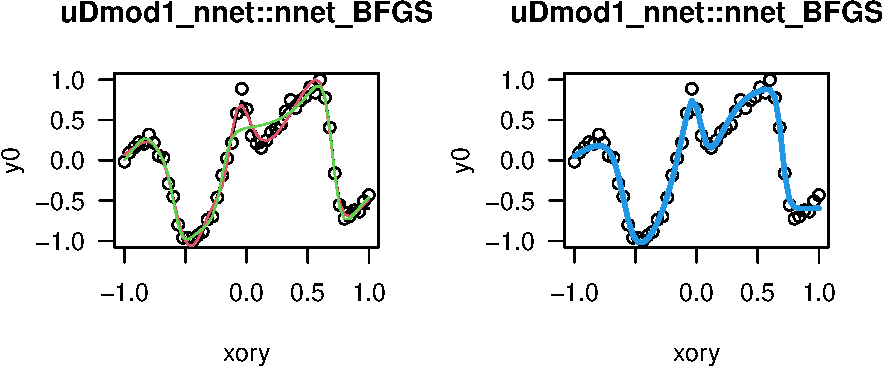
\includegraphics{unnamed-chunk-7-1} 

}

\caption[Example of nnet on uDmod1]{Example of nnet on uDmod1}\label{fig:unnamed-chunk-7}
\end{figure}
\end{Schunk}

\hypertarget{appendix-d}{%
\subsection{Appendix D}\label{appendix-d}}

\begin{Schunk}
\begin{table}[!h]

\caption{\label{tab:unnamed-chunk-8}All convergence scores per package:algorithm sorted by minimum RMSE}
\centering
\fontsize{7}{9}\selectfont
\begin{tabular}[t]{>{}llcllcccc}
\toprule
\multicolumn{2}{c}{ } & \multicolumn{3}{c}{Input parameter} & \multicolumn{2}{c}{RMSE Score} & \multicolumn{2}{c}{Other score} \\
\cmidrule(l{3pt}r{3pt}){3-5} \cmidrule(l{3pt}r{3pt}){6-7} \cmidrule(l{3pt}r{3pt}){8-9}
Package & Algorithm & Input format & Maxit & Learn. rate & median & D51 & MAE & WAE\\
\midrule
\textbf{nlsr} & 41. NashLM & full fmla \& data & 200 & - & 3 & 16 & 3 & 6\\
\cmidrule{1-9}
\textbf{rminer} & 45. nnet\_optim(BFGS) & fmla \& data & 200 & - & 1 & 6 & 1 & 1\\
\cmidrule{1-9}
\textbf{nnet} & 42. optim (BFGS) & x \& y & 200 & - & 2 & 17 & 2 & 3\\
\cmidrule{1-9}
 & 56. optim(BFGS) & x \& y & 200 & - & 4 & 10 & 4 & 5\\

 & 57. optim(CG) & x \& y & 1000 & - & 6 & 10 & 5 & 4\\

 & 58. optim(L-BFGS-B) & x \& y & 200 & - & 13 & 30 & 14 & 13\\

 & 59. optim(Nelder-Mead) & x \& y & 10000 & - & 44 & 45 & 46 & 42\\

\multirow{-5}{*}{\raggedright\arraybackslash \textbf{validann}} & 60. optim(SANN) & x \& y & 1000 & - & 53 & 51 & 56 & 55\\
\cmidrule{1-9}
\textbf{MachineShop} & 32. nnet\_optim(BFGS) & fmla \& data & 200 & - & 9 & 22 & 9 & 7\\
\cmidrule{1-9}
\textbf{traineR} & 55. nnet\_optim(BFGS) & fmla \& data & 200 & - & 5 & 15 & 6 & 2\\
\cmidrule{1-9}
\textbf{radiant.model} & 44. nnet\_optim(BFGS) & "y" \& data & 200 & - & 8 & 32 & 12 & 10\\
\cmidrule{1-9}
 & 34. optimx(BFGS) & x \& y & 200 & - & 10 & 18 & 9 & 11\\

\multirow{-2}{*}{\raggedright\arraybackslash \textbf{monmlp}} & 35. optimx(Nelder-Mead) & x \& y & 10000 & - & 47 & 45 & 44 & 47\\
\cmidrule{1-9}
 & 12. optim(BFGS) & x \& y & 200 & - & 28 & 48 & 21 & 40\\

 & 14. Rprop & x \& y & 1000 & 0.01 & 54 & 60 & 52 & 58\\

\multirow{-3}{*}{\raggedright\arraybackslash \textbf{CaDENCE}} & 13. pso\_psoptim & x \& y & 1000 & - & 56 & 56 & 54 & 56\\
\cmidrule{1-9}
\textbf{h2o} & 24. first-order & "y" \& data & 10000 & 0.01 & 7 & 7 & 8 & 8\\
\cmidrule{1-9}
\textbf{EnsembleBase} & 23. nnet\_optim(BFGS) & x \& y & 200 & - & 15 & 34 & 15 & 15\\
\cmidrule{1-9}
\textbf{caret} & 15. avNNet\_nnet\_optim(BFGS) & x \& y & 200 & - & 10 & 21 & 11 & 9\\
\cmidrule{1-9}
\textbf{brnn} & 11. Gauss-Newton & x \& y & 200 & - & 12 & 9 & 13 & 12\\
\cmidrule{1-9}
\textbf{qrnn} & 43. nlm() & x \& y & 200 & - & 14 & 25 & 7 & 36\\
\cmidrule{1-9}
 & 51. Rprop & x \& y & 1000 & - & 23 & 52 & 25 & 28\\

 & 52. SCG & x \& y & 1000 & - & 17 & 26 & 18 & 19\\

 & 53. Std\_Backpropagation & x \& y & 1000 & 0.1 & 32 & 31 & 31 & 36\\

 & 47. BackpropChunk & x \& y & 1000 & - & 34 & 41 & 32 & 34\\

 & 48. BackpropMomentum & x \& y & 1000 & - & 35 & 39 & 35 & 30\\

 & 49. BackpropWeightDecay & x \& y & 1000 & - & 30 & 43 & 33 & 31\\

 & 46. BackpropBatch & x \& y & 10000 & 0.1 & 48 & 27 & 50 & 48\\

\multirow{-8}{*}{\raggedright\arraybackslash \textbf{RSNNS}} & 50. Quickprop & x \& y & 10000 & - & 58 & 36 & 58 & 57\\
\cmidrule{1-9}
 & 8. trainwgrad\_adam & x \& y & 1000 & 0.01 & 20 & 35 & 16 & 20\\

 & 9. trainwgrad\_RMSprop & x \& y & 1000 & 0.01 & 31 & 50 & 29 & 39\\

\multirow{-3}{*}{\raggedright\arraybackslash \textbf{automl}} & 10. trainwpso & x \& y & 1000 & - & 41 & 49 & 41 & 38\\
\cmidrule{1-9}
\textbf{deepnet} & 20. BP & x \& y & 1000 & 0.8 & 18 & 38 & 24 & 17\\
\cmidrule{1-9}
 & 38. rprop+ & fmla \& data & 100000 & - & 23 & 40 & 23 & 24\\

 & 37. rprop- & fmla \& data & 100000 & - & 21 & 42 & 21 & 18\\

 & 40. slr & fmla \& data & 100000 & - & 39 & 37 & 39 & 46\\

 & 39. sag & fmla \& data & 100000 & - & 49 & 59 & 47 & 52\\

\multirow{-5}{*}{\raggedright\arraybackslash \textbf{neuralnet}} & 36. backprop & fmla \& data & 100000 & 0.001 & 51 & 10 & 49 & 45\\
\cmidrule{1-9}
 & 28. adamax & x \& y & 10000 & 0.1 & 18 & 20 & 20 & 16\\

 & 27. adam & x \& y & 10000 & 0.1 & 28 & 44 & 30 & 25\\

 & 29. nadam & x \& y & 10000 & 0.1 & 39 & 58 & 40 & 41\\

 & 26. adagrad & x \& y & 10000 & 0.1 & 43 & 53 & 42 & 35\\

 & 25. adadelta & x \& y & 10000 & 0.1 & 35 & 19 & 34 & 33\\

 & 31. sgd & x \& y & 10000 & 0.1 & 45 & 47 & 45 & 43\\

\multirow{-7}{*}{\raggedright\arraybackslash \textbf{keras}} & 30. rmsprop & x \& y & 10000 & 0.1 & 55 & 57 & 55 & 54\\
\cmidrule{1-9}
 & 2. ADAPTgdwm & x \& y & 1000 & 0.01 & 22 & 29 & 16 & 26\\

 & 1. ADAPTgd & x \& y & 1000 & 0.01 & 25 & 8 & 26 & 21\\

 & 4. BATCHgdwm & x \& y & 10000 & 0.1 & 33 & 14 & 37 & 27\\

\multirow{-4}{*}{\raggedright\arraybackslash \textbf{AMORE}} & 3. BATCHgd & x \& y & 10000 & 0.1 & 38 & 24 & 42 & 31\\
\cmidrule{1-9}
\textbf{minpack.lm} & 33. Levenberg-Marquardt & full fmla \& data & 200 & - & 16 & 5 & 19 & 14\\
\cmidrule{1-9}
 & 6. rmsprop & x \& y & 1000 & 0.01 & 25 & 33 & 27 & 23\\

 & 5. adam & x \& y & 1000 & 0.01 & 27 & 27 & 28 & 21\\

\multirow{-3}{*}{\raggedright\arraybackslash \textbf{ANN2}} & 7. sgd & x \& y & 1000 & 0.01 & 37 & 22 & 36 & 29\\
\cmidrule{1-9}
 & 16. adam & x \& y & 10000 & 0.4 & 42 & 1 & 38 & 44\\

 & 19. rmsProp & x \& y & 1000 & 0.8 & 46 & 4 & 48 & 50\\

 & 18. momentum & x \& y & 1000 & 0.8 & 52 & 3 & 53 & 51\\

\multirow{-4}{*}{\raggedright\arraybackslash \textbf{deepdive}} & 17. gradientDescent & x \& y & 10000 & 0.8 & 57 & 2 & 57 & 53\\
\cmidrule{1-9}
\textbf{snnR} & 54. SemiSmoothNewton & x \& y & 200 & - & 49 & 13 & 50 & 48\\
\cmidrule{1-9}
\textbf{elmNNRcpp} & 21. ELM & x \& y & - & - & 59 & 55 & 59 & 59\\
\cmidrule{1-9}
\textbf{ELMR} & 22. ELM & fmla \& data & - & - & 60 & 53 & 60 & 60\\
\bottomrule
\multicolumn{9}{l}{\rule{0pt}{1em}\textit{Note: } TOP5 are nlsr:NashLM, rminer:nnet\_optim(BFGS), nnet:optim (BFGS), validann:optim(BFGS), MachineShop:nnet\_optim(BFGS).}\\
\end{tabular}
\end{table}

\end{Schunk}

\begin{Schunk}
\begingroup\fontsize{7}{9}\selectfont

\begin{longtable}[t]{ll>{\raggedright\arraybackslash}p{10cm}}
\caption{\label{tab:unnamed-chunk-9}Review of Discarded Packages}\\
\toprule
Package & Category & Reason to Discard (File(s) and/or function(s))\\
\midrule
\endfirsthead
\caption[]{Review of Discarded Packages \textit{(continued)}}\\
\toprule
Package & Category & Reason to Discard (File(s) and/or function(s))\\
\midrule
\endhead

\endfoot
\bottomrule
\multicolumn{3}{l}{\rule{0pt}{1em}\textit{Note: } AP=Application, CL=Classification, RE=Regression, RE*=?, TS=Time serie, UT=Utility, XX=Other.}\\
\endlastfoot
appnn & AP & Provide a feed forward neural network to predict the amyloidogenicity propensity of polypeptide sequences (DESCRIPTION file)\\
autoencoder & AP & Provide a sparse autoencoder, an unsupervised algorithm that learns useful features from the data its given (::autoencode)\\
BNN & RE* & Use a feed forward neural network to perform regression. It is unclear whether it fits the form of perceptron in the scope. It states that it is intended for variable selection, although how exactly the package would be used to do so is missing. Also the source code is written in C that users of R might not understand. Performance is slow : need 100.000 iterations. (::BNNsel-examples \& abstract of paper)\\
Buddle & CL & Did not include regression in 2019. Unfortunately, the version we tested in 2020 could not be used properly for regression either. See the examples (::TrainBuddle)\\
cld2 & XX & Provide bindings to Google's C++ library CLD2, which detects languages using a Naïve Bayesian classifier. CLD3, which does use neural networks, is mentioned in the description (DESCRIPTION file \& link to github)\\
\addlinespace
cld3 & AP & Bindings to Google's C++ library CLD3, which detects languages using a neural network with an experimental algorithm (DESCRIPTION file)\\
condmixt & AP & Use neural networks to predict parameters of mixture models (DESCRIPTION file)\\
DamiaNN & RE & Was designed specificly for training datasets from Numerai, <https://numer.ai/>. We were unable to adapt it to our datasets even after exporting functions from the interactive interface (DESCRIPTION file, help pages)\\
deep & CL & Seem to implement a perceptron to classify data (implicitly known from choice of iris as example and in source code)\\
deepNN & RE & Another implementation of deep learning. Its input format of lists of vectors is not standard require users to understand how to use lapply or other functions to convert the format of their data. Univariate datasets can't be used with the functions and we could not manage to adapt it to 2020 code (::train).\\
\addlinespace
DNMF & XX & Help extract features that enforce spatial locality with separability between classes in a discriminant manner (DESCRIPTION file)\\
evclass & CL & Provide an evidential neural network that outputs Dempster-Shafer mass functions (DESCRIPTION file)\\
gamlss.add & UT & Allow users to use nnet with a variety of Generalized Additive Models for Location Scale and Shape (::nn). It is not particularly appropriate for all our datasets.\\
gcForest & XX & Based on an article with "Towards an Alternative to Deep Neural Networks" in its title (DESCRIPTION file)\\
GMDH & TS & Provide GMDH type neural network algorithms for short term forecasting on a univariate time series (DESCRIPTION file)\\
\addlinespace
GMDH2 & CL & Provide GMDH type neural network algorithms for performing binary classification (DESCRIPTION file)\\
GMDHreg & RE* & Regression using GMDH algorithms. We only managed to tested the COMBI algorithm (the most basic and first in the vignette) on the multivariate datasets. It is strangely slow on the "easy" datasets, mFriedman and mRef153. The convergence is relatively not good considering the ammount of layers (Title in DESCRIPTION file)\\
gnn & AP & Out of scope: Generative moment matching networks (GMMNs) are introduced for generating quasi-random samples from multivariate models (article abstract)\\
grnn & RE & Provide an implementation of Specht's General Regression Neural Network in 1991 (DESCRIPTION file). We could not manage to make the functions work on the multivariate datasets. ::guess, the function for predicting, only allows for 1 data at a time. Performance of General Regression Neural Networks can be seen from package yager instead.\\
hybridEnsemble & RE & Hybrid ensemble of eight different sub-ensembles (DESCRIPTION file)\\
\addlinespace
image.libfacedetection & AP & Face detection with CNNs (DESCRIPTION file)\\
isingLenzMC & AP & Out of scope: This package provides utilities to simulate one dimensional Ising Model with Metropolis and Glauber Monte Carlo (DESCRIPTION file)\\
kerasR & RE & See section on keras\\
leabRa & RE & Provide the local error driven and associative biologically realistic algorithm (Leabra) from O'Reilly 1996. It combines supervised and unsupervised learning, so out of scope (DESCRIPTION file).\\
learNN & CL & Implement some basic neural networks from \textbackslash{}url\{http://qua.st/\} (DESCRIPTION file). Examples seem to focus on binary classification (::learn\_gd, ::learn\_bp).\\
\addlinespace
LilRhino & AP & Provide binary neural networks meant for reducing data (DESCRIPTION file), a random forest style collection of neural networks for classification (::Random\_Brains), and code for even more purposes. Documentation is satisfyingly clear for a package for applications: a 3 layer network with an adam optimizer, with an explanation of its activation functions (::Binary\_Network)\\
neural & CL & An implementation of "a simple MLP neural network that is suitable for classification tasks" (::mlptrain)\\
NeuralNetTools & UT & Out of scope: Functions are available for plotting, quantifying variable importance, conducting a sensitivity analysis, and obtaining a simple list of model weights (DESCRIPTION file and Help Pages titles)\\
NeuralSens & UT & A greater focus on sensitivity, with additional functions (DESCRIPTION file)\\
NlinTS & TS & A non-linear version of a causality test with feed forward neural networks and a Vector Auto-Regressive Neural Network (VARNN) for non-linear time series analysis models (DESCRIPTION file)\\
\addlinespace
nnetpredint & UT & Out of scope: Computing prediction intervals of neural network models at certain confidence level (DESCRIPTION file)\\
nnfor & TS & Automatic to fully manual time series modelling with neural networks (DESCRIPTION file)\\
nnlib2Rcpp & CL & Provide a collection of neural networks, but examples seem to indicate classification and testing our code with the functions provided led to error. Using the RcppClass might be confusing for less experienced R users (::NN-class)\\
nntrf & AP & Provide useful pre-processing for Machine Learning tasks through data transformation in a non-linear, supervised way with a perceptron (DESCRIPTION file)\\
onnx & UT & Aims to provide an open source format for neural networks, with definitions of an extensible computation graph model, built-in operators, and standard data types (DESCRIPTION file)\\
\addlinespace
OptimClassifier & UT & Search for the best amount of neurons for binary classifcation neural networks, among other types of binary classifiers (based on how Optim.NN works \& DESCRIPTION file)\\
OSTSC & UT & A tool to solve imbalanced data for univariate time series classification with oversampling using integrated ESPO and ADASYN methods (DESCRIPTION file) thus improving the performance of RNN classifiers (vignette)\\
passt & AP & This package provides implementation of the Probability Associator Time (PASS-T) model, a memory model based on a simple competitive artificial neural network which imitates human judgment of frequency and duration (DESCRIPTION file)\\
pnn & CL & This package provides implementation of the Specht algorithm, 1990, for classification with four functions: learn, smooth, perf, and guess (DESCRIPTION file)\\
polyreg & XX & Polyregression as alternative to NN (DESCRIPTION file)\\
\addlinespace
predictoR & RE & A shiny interface for supervised learning with very minimal documentation. Users may be additionally confused when opening the application only to find that it's default language is Espanol, although this can be changed in the Idioma section. (DESCRIPTION file \& ::init\_predictor)\\
ProcData & AP & Provide tools for exploratory process data analysis via functions: reading, process manipulation, action sequence generators, feature extraction and prediction (link + DESCRIPTION file)\\
quarrint & AP & Out of scope: provide two indexes for interaction prediction between groundwater and quarry extension, one of which is an artificial neural network ; specified classifier for quarry data (help page - quarrint-package and DESCRIPTION file)\\
rasclass & CL & Provide neural networks as one of the five supervised classification algorithms for raster images with a design meant to facilitate land-cover analysis (DESCRIPTION file)\\
rcane & RE & Provide parameter estimation for linear regression, which was not appropriate for the relationships in our data. (DESCRIPTION file)\\
\addlinespace
regressoR & RE & A manual rich version of predictoR\\
rnn & AP & Implementations of the vanilla Recurrent Neural Network, Long Short-Term Memory (LSTM), and Gated Recurrent Unit (GRU) in native R (DESCRIPTION file)\\
RTextTools & AP & Out of scope: A machine learning package for automatic text classification (DESCRIPTION file)\\
ruta & AP & unsupervised neural networks (DESCRIPTION file)\\
simpleNeural & CL & Neural networks for multi-class or binary classification (DESCRIPTION file)\\
\addlinespace
softmaxreg & CL & Out of scope: Implementation of 'softmax' regression and classification models with multiple layer neural network (DESCRIPTION file)\\
Sojourn.Data & AP & Stores some neural networks used for Sojourn Accelerometer methods (DESCRIPTION file)\\
spnn & CL & Out of scope : Scale invariant version of the original PNN with the added functionality of allowing for smoothing along multiple dimensions while accounting for covariances within the data set (DESCRIPTION file)\\
studyStrap & AP & Implements multi-study learning algorithms such as merging, the study-specific ensemble the study strap, the covariate-matched study strap, covariate-profile similarity weighting, and stacking weights with single-study learners from caret (DESCRIPTION file)\\
TeachNet & CL & Provide neural networks with up to 2 hidden layers, 2 different error functions, and a weight decay for 2 class classification : it is slow. (DESCRIPTION file \& ::TeachNet)\\
\addlinespace
tensorflow & RE & See section on keras\\
tfestimators & RE & See section on keras\\
trackdem & AP & An artificial neural network can be trained for filtering false positives present in video materials or image sequences (DESCRIPTION file)\\
TrafficBDE & RE* & Use caret for a grid of parameters for 3 layers combined with neuralnet. Is very slow. Out of scope to test one layer perceptrons. We recommend the author to use other packages and lessen the number of layers. Datasets in Traffic Status Prediction and Urban Places are similar in nature to ours (TrainCR.R, DESCRIPTION file)\\
tsfgrnn & TS & Out of scope: A general regression neural network (GRNN) is a variant of a Radial Basis Function Network. Allow you to forecast time series using an autoregressive GRNN model (DESCRIPTION file)\\
\addlinespace
yager & RE* & This package provides a neural network that behaves differently from a perceptron. Results indicate that predictions are quite close to the real values, however this comes at the cost of a large number of weights. With less weights or insufficient training data, the performance isn't as great. (::grnn.fit)\\
yap & CL & Yet another PNN, with a N-level response, where N > 2 (DESCRIPTION file)\\
zFactor & AP & Computational algorithms to solve equations and find the 'compressibility' factor `z` of hydrocarbon gases (DESCRIPTION file)\\*
\end{longtable}
\endgroup{}

\end{Schunk}


\address{%
Salsabila Mahdi\\
Universitas Syiah Kuala\\%
JL. Syech Abdurrauf No.3, Aceh 23111, Indonesia\\
%
%
\\\textit{ORCiD: \href{https://orcid.org/0000-0002-2559-4154}{0000-0002-2559-4154}}%
\\\href{mailto:bila.mahdi@mhs.unsyiah.ac.id}{\nolinkurl{bila.mahdi@mhs.unsyiah.ac.id}}
}

\address{%
Akshaj Verma\\
Manipal Institute of Technology\\%
Manipal, Karnataka, 576104, India\\
%
%
\\\textit{ORCiD: \href{https://orcid.org/0000-0002-3936-0033}{0000-0002-3936-0033}}%
\\\href{mailto:akshajverma7@gmail.com}{\nolinkurl{akshajverma7@gmail.com}}
}

\address{%
Christophe Dutang\\
Université Paris-Dauphine, University PSL, CNRS, CEREMADE\\%
Place du Maréchal de Lattre de Tassigny, 75016 Paris, France\\
%
%
\\\textit{ORCiD: \href{https://orcid.org/0000-0001-6732-1501}{0000-0001-6732-1501}}%
\\\href{mailto:dutang@ceremade.dauphine.fr}{\nolinkurl{dutang@ceremade.dauphine.fr}}
}

\address{%
Patrice Kiener\\
InModelia\\%
5 rue Malebranche, 75005 Paris, France\\
%
%
\\\textit{ORCiD: \href{https://orcid.org/0000-0002-0505-9920}{0000-0002-0505-9920}}%
\\\href{mailto:patrice.kiener@inmodelia.com}{\nolinkurl{patrice.kiener@inmodelia.com}}
}

\address{%
John C. Nash\\
Telfer School of Management, University of Ottawa\\%
55 Laurier Avenue East, Ottawa, Ontario K1N 6N5 Canada\\
%
%
\\\textit{ORCiD: \href{https://orcid.org/0000-0002-2762-8039}{0000-0002-2762-8039}}%
\\\href{mailto:nashjc@uottawa.ca}{\nolinkurl{nashjc@uottawa.ca}}
}
